%!TEX root = ../tcc.tex

\chapter{Anatomia do BitTorrent}

O BitTorrent é uma rede \gls{p2p} onde cada um de seus usuários assume o papel híbrido
de servidor, que fornece os arquivos, e de cliente, que adquire os arquivos. Cada
computador é chamado de \gls{peer}.

Cada transferência por BitTorrent está associada a um arquivo de \glspl{metadata}
chamado \gls{torrent}. Esse arquivo contém informações sobre os arquivos que formam o
pacote de dados daquele conjunto de dados e também um ou mais endereços de
\glspl*{tracker}, que mantém listas atualizadas dos \glspl*{peer} que estão
compartilhando os dados, atualizado em períodos de tempo curtos (usualmente 30 minutos).

Enquanto um \gls*{peer} estiver fazendo download de um \gls*{torrent} é chamado de
\gls{leecher}, pois ainda estará consumindo dados de outros \glspl*{peer}; quando o
download acabar, passará a ser um \gls{seeder}, que somente envia dados para outros
\glspl*{peer}.

\Glspl*{peer} que participam do compartilhamento de um arquivo \gls*{torrent} específico
fazem parte do \gls{swarm}, onde os dados contidos no pacote desse arquivo são
compartilhados com os outros de forma independente e paralela por partes.

\begin{figure}
    \centering
    \begin{subfigure}[b]{0.3\textwidth}
            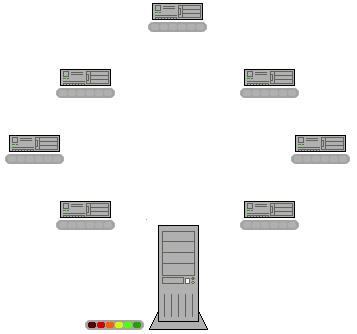
\includegraphics[width=\textwidth]{multiple/Torrentcomp_small-0.png}
            \caption{A gull}
            \label{fig:gull}
    \end{subfigure}%
    ~ %add desired spacing between images, e. g. ~, \quad, \qquad etc.
      %(or a blank line to force the subfigure onto a new line)
    \begin{subfigure}[b]{0.3\textwidth}
            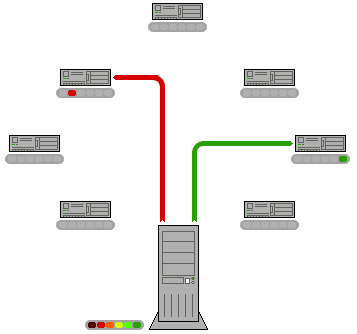
\includegraphics[width=\textwidth]{multiple/Torrentcomp_small-1.png}
            \caption{A tiger}
            \label{fig:tiger}
    \end{subfigure}
    ~ %add desired spacing between images, e. g. ~, \quad, \qquad etc.
      %(or a blank line to force the subfigure onto a new line)
    \begin{subfigure}[b]{0.3\textwidth}
            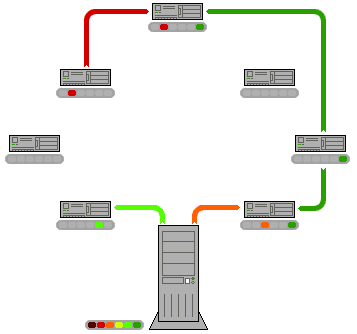
\includegraphics[width=\textwidth]{multiple/Torrentcomp_small-2.png}
            \caption{A mouse}
            \label{fig:mouse}
    \end{subfigure}
    \caption{Pictures of animals}\label{fig:animals}
\end{figure}


\section{Busca por informações}

Os arquivos \gls*{torrent} ficam disponíveis em vários sites de índice, como o
\href{http://thepiratebay.sx/}{ThePirateBay}, o \href{http://kickass.to/}{Kickass} ou
\href{https://torrentz.eu/}{Torrentz}, muitas vezes em mais de um deles ao mesmo tempo.
Apesar de todo conteúdo compartilhado possuir um arquivo \gls*{torrent}, não
necessariamente um arquivo \gls*{torrent} está sendo compartilhado, podendo inclusive
estar extinto. Por questões didáticas, usaremos um arquivo torrent do filme `A Noite
dos Mortos Vivos' de 1960 \cite{torrent-file}, que é de domínio público e livre de
direitos autorais.

Se abrirmos esse arquivo, veremos um conteúdo ilegível de forma compacta. Após tratar o
conteúdo, obtemos o seguinte (parcialmente apagado para questões de formatação):
\todoquestion{tudo bem fazer isso? preciso anexar o arquivo completo?}

\begin{minted}[
    linenos,
    frame=single,
    numbersep=6pt,
    baselinestretch=1,
    fontfamily=courier,
    fontsize=\tiny
]{text}
d
    8:announce
    36:http://bt1.archive.org:6969/announce
    13:announce-list
    l
        l36:http://bt1.archive.org:6969/announcee
        l36:http://bt2.archive.org:6969/announcee
    e
    7:comment
    13:creation date
    i1343715473e
    4:info
    d
        5:files
        l
            d
                5:crc32
                8:030208fe
                6:length
                i4127671704e
                3:md5
                32:627f5a428f9e454ccfcb29d31b87169a
                5:mtime
                10:1079402480
                4:path
                l29:night_of_the_living_dead.mpege
                4:sha1
                40:5e44bb1b3f700240249a5287c64dc02dc56d034b
            e
        e
        4:name
        24:night_of_the_living_dead
        12:piece length
        i4194304e
        6:pieces
        23720:<binary>
    e
    6:locale
    2:en
    5:title
    24:night_of_the_living_dead
    8:url-list
    l
        28:http://archive.org/download/
        39:http://ia600301.us.archive.org/22/items
        39:http://ia700301.us.archive.org/22/items
    e
e
\caption{Exemplo de conteúdo de arquivo .torrent}
\end{minted}

continua...

\todo[inline]{explicar isso \cite{site:torrent-spec-wiki}}

\section{Fontes de arquivos}

Mostrarei o processamento dos dados adquiridos na seção anterior e como ele organiza a lista das fontes de arquivos usando a tabela hash DHT Kademlia.

\section{Jogo da troca de arquivos}

Explicarei o algoritmo tit-for-tat padrão do protocolo BitTorrent, que vem da Teoria dos Jogos, e como o Transmission o implementa.

\afterpage{\clearpage}